\section{Cortes Clique}

\bigskip
\subsection{Formulaci\'on}

Lo cortes clique como el nombre lo indica requieren alg\'un grafo subyacente del cual se puedan inferir cortes.
Antes de explicar los cortes, vamos a comentar el grafo de nuestro problema.

Las instancias a resolver fueron restringidas a instancias con todas las variables binarias.
Existen grafos que sirven para representar este tipo de problemas y son los grafos de conflictos.
Lo que nos dice el grafo de conflicto es si existen combinaciones de pares de nodos que no pueden ocurrir, es decir,
dadas las restricciones de nuestro problema puede existir variables $x_2$ y $x_3$ tal que que si las dos estan en 1,
el conjunto de restricciones se vuelve infactible(como en la ecuaci\'on 1). De la misma manera puede ocurrir que $x_2$ este en 1, y $x_1$ esta en 0 y que tambien
as\'i el conjunto de resticciones sea infactible (como en la ecuaci\'on 2).

\begin{equation}
-3 x_1 + 3 x_2 + 5 x_3 \leq 3
\end{equation}
\begin{equation}
4 x_1 - 1 x_2 + 3 x_3 \geq 3
\end{equation}

Por lo tanto, existen combinaciones de pares de nodos que no pueden ocurrir en nuestro problema, cada combinaci\'on que no pueda ocurrir
es un eje en nuestro grafo de conflictos. Para representar este grafo, tenemos un conjunto $\mathcal{V}$ dos nodos por cada variable, $x_i$
representando la variable $x_i$ en 1, y $\tilde{x}_i$ para la variable $x_i$ en 0. Por lo tanto, nuestro conjunto $\mathcal{E}$ de ejes son los pares de 
nodos que no pueden ocurrir en nuestro problema, entre ellos, los que conectan a $x_i$ con $\tilde{x}_i$ como muestra la FIGURA1.


\begin{figure}[H]
\begin{center}
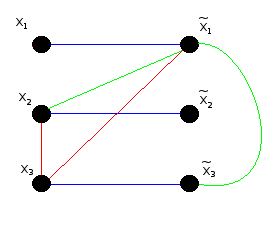
\includegraphics{grafoconflicto}
\end{center}
\label{Grafo de conflictos del las restricciones REF}
\end{figure}

Una vez que tenemos armado el grafo, se puede ver que las soluciones factibles, son en realidad conjuntos independientes en nuestro grafo
(ie: no existen dos nodos conectados con un eje, porque estan conectas las que hacen problema infactible). Por lo tanto cada eje representa
tambi\'en una restricci\'on en el problema dependiendo la combinaci\'on variables.

\begin{itemize}
\item Si los nodos $x_i$ y $x_j$ son vecinos tenemos una restricci\'on del estilo $x_i +x_j \leq 1$
\item Si los nodos $x_i$ y $\tilde{x}_j$ son vecinos tenemos una restricci\'on del estilo $x_i + 1-x_j \leq 1$
\item Si los nodos $\tilde{x}_i$ y $x_j$ son vecinos tenemos una restricci\'on del estilo $1-x_i +x_j \leq 1$
\item Si los nodos $\tilde{x}_i$ y $\tilde{x}_j$ son vecinos tenemos una restricci\'on del estilo $1-x_i + 1-x_j \leq 1$
\end{itemize}

Una idea ingenua podria insertar todos estas restricciones a nuestro problema, reduciendo as\'i la posibilidad de que tener soluciones no factibles.
Pero al aumentar la cantidad de resticciones considerablemente, se tarda m\'as en resolver el problem por el m\'etodo simplex. Por lo que vamos
a insertar las restricciones a medida que resulten convenientes.

Cuando resulta conveniente? Si en la relajaci\'on lineal se viola alguna restricci\'on, va a ser conveniente cortar soluciones de ese tipo.
Como la soluci\'on ser\'a un conjunto indepentiente en el grafo de conflictos, entonces, todas las cliques en nuestro grafo tienen a lo sumo
un nodo como parte de la soluci\'on. Entonces si al encontrar la relajaci\'on lineal encontramos una clique que viole esta condici\'on, entonces
insertamos la resticci\'on de la clique a nuestro problema.

\begin{equation}
\sum\limits_{i \in \mathcal{K}} x_i \leq 1
\end{equation}

\bigskip
\subsection{Construcci\'on del grafo}

Lo primero que debemos hacer por lo tanto es construir el grafo de conflictos que mencionamos en la secci\'on anterior (<-REFERNCIA COPADA).
Si la instancia del problema lo permite, realizamos fuerza bruta sobre todas las posibilidades. Es decir, para cada par de variables y para cada 
combinaci\'on de variable en 1 y variable en 0, buscamos si el conjunto de restricciones es infactible.

Para ver si el conjunto de restricciones es factible dado que tenemos dos variables que sabemos que tienen un valor fijo, lo que hacemos es buscar
todas las restricciones que contengan a estas dos variables y ver si existe una valuaci\'on tal que sea factible. Esto se puede hacer de manera
golosa, ya que la resticciones que son por menor o igual, basta poner en 1 todas las variables con coeficiente negativo, y en 0 todas las variables que tengan coeficiente positivo. Si usando
esta valuaci\'on la restricci\'on resulta infactible se puede probar que el conjunto de restricciones es infactible para esta combinaci\'on de nodos. De manera analoga para las resticciones
 por mayor o igual, intentaremos que las variables que tengan coeficiente positivo esten en 1, y las dem\'as en 0 (recordando que hay 2 nodos cuyo valor es fijo).

Para los casos donde no sea posible (ya sea porque hay demasiados ejes en el grafo de conflictos, o porque tarda demasiado). Lo que hacemos es quedarnos
con un conjunto al azar de variables, y probar sobre estas si existen ejes.

\bigskip
\subsection{Algoritmo de separaci\'on}


buscar es clique es np-conchatuma

generamos clique maximales

heuristica

ordenamos por mayor de xestrella, vamos agarrando los mas grandes que tienen ejes con todos los anteriores voila
